\begin{figure}
	\centering
	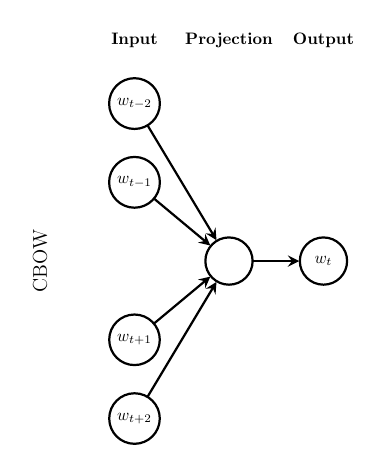
\begin{tikzpicture}[
		scale=0.4,
		every node/.style={scale=0.6},
		n/.style={circle,draw=black,thick,minimum width=1cm},
		arr/.style={-stealth,thick}
	]

		\node[rotate=90] at (-6,0) {\highlight{\large CBOW}};

		% input
		\node at (-3,7) {\textbf{Input}};
		\node[n] (I1) at (-3,5) {$\bm{w}_{t-2}$}; 
		\node[n] (I2) at (-3,2.5) {$\bm{w}_{t-1}$};
		\node[n] (I3) at (-3,-2.5) {$\bm{w}_{t+1}$}; 
		\node[n] (I4) at (-3,-5) {$\bm{w}_{t+2}$};
		
		% projection
		\node at (0,7) {\textbf{Projection}};
		\node[n] (P1) at (0,0) {};
		
		% output
		\node at (3,7) {\textbf{Output}};
		\node[n] (O1) at (3,0) {$\bm{w}_t$};

		% connections
		\draw[arr] (I1) -- (P1); \draw[arr] (I2) -- (P1); \draw[arr] (I3) -- (P1); \draw[arr] (I4) -- (P1);
		\draw[arr] (P1) -- (O1);

	\end{tikzpicture}
\end{figure}